\documentclass[preprint,12pt,aps,pra,showkeys,amsmath,amssymb,superscriptaddress,floatfix]{revtex4-2}
\usepackage[T1]{fontenc}
\usepackage[utf8]{inputenc}
\usepackage{amsmath,amssymb,amsthm,mathtools,mathrsfs}
\usepackage{microtype,booktabs,enumitem}
\usepackage{xcolor,tikz,etoolbox}
\usepackage[skins,breakable]{tcolorbox}
\usepackage{needspace}
% Keep diagram geometry independent of REVTeX preprint body spacing.
\AtBeginEnvironment{tikzpicture}{\linespread{1}\selectfont}
\usetikzlibrary{arrows.meta,positioning,calc,fit,decorations.pathreplacing}
\usepackage{graphicx}
\usepackage{hyperref}

\definecolor{MMBlue}{RGB}{0,82,155}
\definecolor{MMOrange}{RGB}{200,80,0}
\tikzset{
 mmnode/.style={draw=MMBlue,rounded corners=2pt,fill=MMBlue!4,align=left,execute at begin node={\raggedright},text width=5cm,font=\fontsize{10}{12}\selectfont,inner sep=6pt},
 mmimport/.style={mmnode,draw=black!65,fill=black!4},
 mmcandidate/.style={mmnode,draw=MMOrange,dashed,fill=MMOrange!5},
 mmrejected/.style={mmnode,draw=black,densely dotted,fill=black!8},
 mmproof/.style={->,thick,MMBlue},
 mmflow/.style={->,semithick,black!70},
 mmrepair/.style={->,dashed,thick,MMOrange},
 mmcandidatearrow/.style={->,dashed,semithick,MMOrange},
 mmnote/.style={font=\scriptsize,fill=white,inner sep=2pt,align=center}}

\usepackage[section]{placeins}
\setlength{\emergencystretch}{3em}
\setlist{itemsep=3pt,topsep=4pt}
\newtheorem{theorem}{Theorem}[section]
\newtheorem{proposition}[theorem]{Proposition}
\newtheorem{lemma}[theorem]{Lemma}
\newtheorem{corollary}[theorem]{Corollary}
\theoremstyle{definition}
\newtheorem{definition}[theorem]{Definition}
\newtheorem{example}[theorem]{Example}
\theoremstyle{remark}
\newtheorem{remark}[theorem]{Remark}
% Avoid isolated statement headings and single-line paragraph fragments.
\BeforeBeginEnvironment{theorem}{\Needspace{6\baselineskip}}
\BeforeBeginEnvironment{definition}{\Needspace{5\baselineskip}}
\BeforeBeginEnvironment{proposition}{\Needspace{5\baselineskip}}
\BeforeBeginEnvironment{lemma}{\Needspace{5\baselineskip}}
\BeforeBeginEnvironment{corollary}{\Needspace{5\baselineskip}}
\clubpenalty=5000
\widowpenalty=5000
\newcommand{\R}{\mathbb R}\newcommand{\Z}{\mathbb Z}\newcommand{\N}{\mathbb N}
\newcommand{\Pa}{\operatorname{Pa}}\newcommand{\Desc}{\operatorname{Desc}}
\newcommand{\cl}{\operatorname{cl}}\newcommand{\cost}{\operatorname{cost}}
\newcommand{\status}{\operatorname{status}}
% Faculty cards: a visual rail groups the five faculties within one agent.
% The rail has no arrowhead and does not represent a proof dependency.
\newcommand{\mmfacultybadge}[1]{%
 \node[circle,draw=MMBlue,line width=1pt,fill=white,
 minimum size=7mm,inner sep=0pt,font=\sffamily\small\bfseries,text=MMBlue]
 at ([xshift=15pt,yshift=-15pt]frame.north west) {#1};}
\newcommand{\mmfacultyrail}{%
 \draw[MMBlue!80,line width=1pt]
 ([xshift=15pt,yshift=2pt]frame.north west)--
 ([xshift=15pt,yshift=-2pt]frame.south west);}
\newtcolorbox{mmfacultybox}[2]{enhanced,breakable,
 colback=MMBlue!4,colframe=MMBlue!4,boxrule=0pt,arc=3pt,
 left=39pt,right=9pt,top=4pt,bottom=4pt,
 before skip=2pt,after skip=2pt,
 fontupper=\small\linespread{1.1}\selectfont,
 overlay unbroken={\mmfacultyrail\mmfacultybadge{#1}},
 overlay first={\mmfacultyrail\mmfacultybadge{#1}},
 overlay middle={\mmfacultyrail},overlay last={\mmfacultyrail}}
\newcommand{\mmfaculty}[3]{%
 \begin{mmfacultybox}{#1}{#2}
 {\sffamily\bfseries\color{MMBlue}#2}\par\smallskip #3
 \end{mmfacultybox}}
\newcommand{\agent}[9]{%
 \Needspace{8\baselineskip}
 \subsubsection{#1}
 \noindent\textbf{Object.} #2\par
 \noindent\textbf{Role.} #3\par\smallskip
 \mmfaculty{E}{Ego}{#4}
 \mmfaculty{M}{Memory}{#5}
 \mmfaculty{I}{Intellect}{#6}
 \mmfaculty{S}{Sense}{#7}
 \mmfaculty{A}{Action}{#8}
 \smallskip\noindent #9\par}

\usepackage{longtable,array,calc}
\providecommand{\tightlist}{\setlength{\itemsep}{2pt}\setlength{\parskip}{0pt}}
\makeatletter
\def\frontmatter@abstract@produce{\par\addvspace{\frontmatter@preabstractspace}%
\begingroup\prep@absbox\unvbox\absbox\post@absbox\endgroup
\addvspace{\frontmatter@postabstractspace}}
\makeatother
\newcommand{\field}[2]{\par\smallskip\noindent\textbf{#1.} #2\par}
\setlength{\emergencystretch}{5em}
\AtBeginEnvironment{verbatim}{\small\linespread{1.0}\selectfont}


\hypersetup{colorlinks=true,linkcolor=MMBlue,urlcolor=MMBlue,pdfauthor={Dibakar Sigdel}}

\begin{document}

\title{Hopf--Rinow Theorem\\[4pt]\large An End-to-End Meta-Math Walkthrough}

\author{Dibakar Sigdel}

\affiliation{Mindverse Computing LLC, Lynnwood, WA 98087, USA}

\date{October 2026}

\begin{abstract}

A complete authored walkthrough of hopf--rinow theorem, with explicit
mathematical contracts, local verification gates, and reusable exports.
The report presents the target theorem, declared imports, a dependency
graph, five-faculty node contracts, a continuous proof, a worked
example, and a hypothesis-repair audit. It is an authored mathematical
exposition, not a deployed-agent transcript or a formal proof-assistant
certificate.

\end{abstract}\maketitle\linespread{1.12}\selectfont

\noindent\textbf{DG-05 / Differential Geometry / Report v1}

\section{Target and import contract}

\begin{theorem}

For a connected finite-dimensional Riemannian manifold without boundary,
prove equivalence of metric completeness, geodesic completeness, and
compactness of every closed bounded subset. Deduce that metric
completeness guarantees a minimizing geodesic between any two points.

\end{theorem}

\subsection{Foundations and permitted imports}

The Riemannian distance is the infimum of piecewise smooth path lengths
on a connected finite-dimensional smooth manifold without boundary.
Import normal-neighborhood geometry and Gauss lemma: sufficiently small
radial geodesics minimize length and small metric spheres are compact
images of tangent spheres. Import local geodesic ODE
existence/uniqueness and the no-corner lemma: a piecewise geodesic that
realizes the distance is smooth at its joins (first variation shortens a
nonzero corner). These local facts do not assert global completeness or
global minimizer existence.

For the minimizing-direction construction fix \(p\ne q\) and write
\(r=d(p,q)>0\). When proving the implication from geodesic completeness,
assume that condition directly; N1 is needed only to obtain it from
metric completeness.

\clearpage\section{Node interaction workflow}

\begin{center}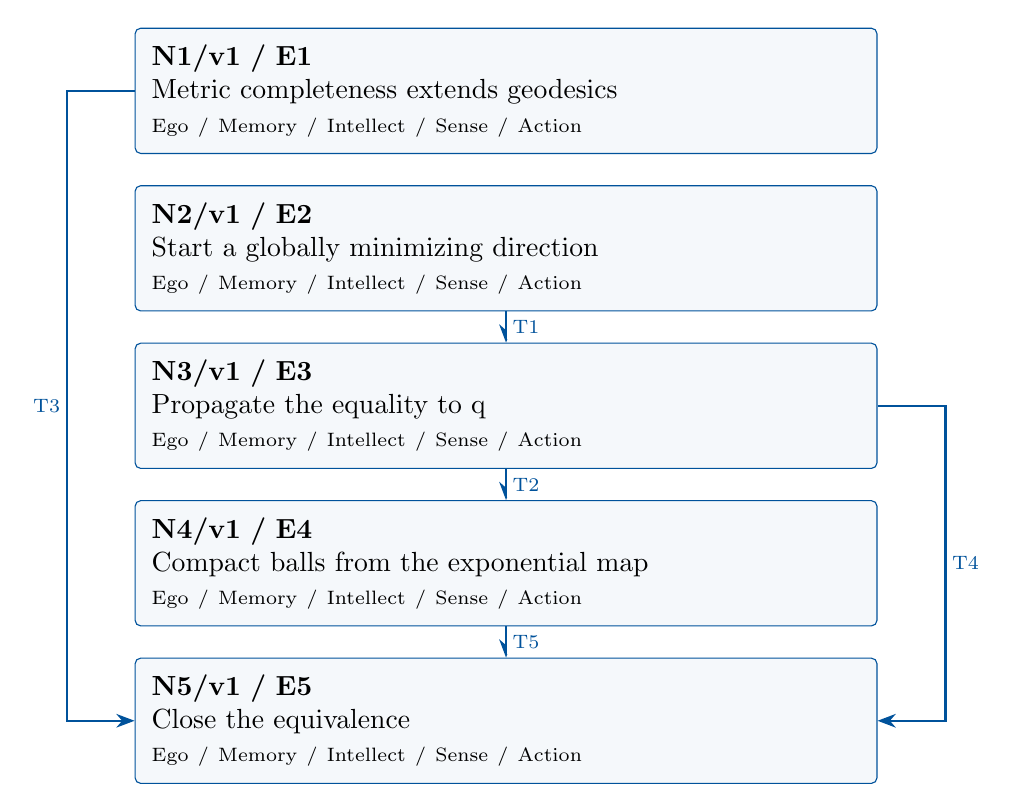
\begin{tikzpicture}[>=Stealth,x=1cm,y=1cm]

\node[mmnode,text width=9cm,minimum height=1.25cm] (N1) at (0,0.0) {\textbf{N1/v1 / E1}\\Metric completeness extends geodesics\\{\scriptsize Ego / Memory / Intellect / Sense / Action}};

\node[mmnode,text width=9cm,minimum height=1.25cm] (N2) at (0,-2.0) {\textbf{N2/v1 / E2}\\Start a globally minimizing direction\\{\scriptsize Ego / Memory / Intellect / Sense / Action}};

\node[mmnode,text width=9cm,minimum height=1.25cm] (N3) at (0,-4.0) {\textbf{N3/v1 / E3}\\Propagate the equality to q\\{\scriptsize Ego / Memory / Intellect / Sense / Action}};

\node[mmnode,text width=9cm,minimum height=1.25cm] (N4) at (0,-6.0) {\textbf{N4/v1 / E4}\\Compact balls from the exponential map\\{\scriptsize Ego / Memory / Intellect / Sense / Action}};

\node[mmnode,text width=9cm,minimum height=1.25cm] (N5) at (0,-8.0) {\textbf{N5/v1 / E5}\\Close the equivalence\\{\scriptsize Ego / Memory / Intellect / Sense / Action}};

\draw[mmproof] (N2.south) -- node[mmnote,right] {T1} (N3.north);

\draw[mmproof] (N3.south) -- node[mmnote,right] {T2} (N4.north);

\draw[mmproof] (N1.west) -- (-5.58,0) -- node[mmnote,left] {T3} (-5.58,-8) -- (N5.west);

\draw[mmproof] (N3.east) -- (5.58,-4) -- node[mmnote,right] {T4} (5.58,-8) -- (N5.east);

\draw[mmproof] (N4.south) -- node[mmnote,right] {T5} (N5.north);

\end{tikzpicture}\end{center}

Each box is one mathematical agent containing all five faculties. Blue
arrows carry the versioned exports listed below. The layout gives a
reading order; only drawn arrows assert dependencies. Diagnostic repair
is separate from the proof DAG.

\clearpage\subsection{Versioned evidence-transfer ledger}

\begingroup\small\linespread{1.05}\selectfont

\Needspace{5\baselineskip}\field{T1: N2/E2/v1 to N3}{A radial geodesic with the distance equality at a positive time.}

\field{Receiving activity}{N3: Propagate the equality to q}

\field{Compatibility}{Use the same mathematical objects and hypotheses as the source export.
Receiving contract: The globally defined radial \(\gamma\) and local
compact spheres; prior exports E2/v1}

\Needspace{5\baselineskip}\field{T2: N3/E3/v1 to N4}{Geodesic completeness implies a minimizing geodesic for every p,q.}

\field{Receiving activity}{N4: Compact balls from the exponential map}

\field{Compatibility}{Use the same mathematical objects and hypotheses as the source export.
Receiving contract: Geodesic completeness and global minimizers; prior
exports E3/v1}

\Needspace{5\baselineskip}\field{T3: N1/E1/v1 to N5}{Metric completeness implies geodesic completeness.}

\field{Receiving activity}{N5: Close the equivalence}

\field{Compatibility}{Use the same mathematical objects and hypotheses as the source export.
Receiving contract: Compact closed bounded subsets; prior exports E1/v1,
E3/v1, E4/v1}

\Needspace{5\baselineskip}\field{T4: N3/E3/v1 to N5}{Geodesic completeness implies a minimizing geodesic for every p,q.}

\field{Receiving activity}{N5: Close the equivalence}

\field{Compatibility}{Use the same mathematical objects and hypotheses as the source export.
Receiving contract: Compact closed bounded subsets; prior exports E1/v1,
E3/v1, E4/v1}

\Needspace{5\baselineskip}\field{T5: N4/E4/v1 to N5}{Geodesic completeness implies compactness of every closed bounded
subset.}

\field{Receiving activity}{N5: Close the equivalence}

\field{Compatibility}{Use the same mathematical objects and hypotheses as the source export.
Receiving contract: Compact closed bounded subsets; prior exports E1/v1,
E3/v1, E4/v1}

\endgroup

\clearpage\section{Agent roles and five-faculty activities}\begingroup\small\linespread{1.05}\selectfont\setlist{itemsep=1pt,topsep=2pt}

\subsection{N1/v1: Metric completeness extends geodesics}

\field{Object and role}{Take a metric endpoint then apply local ODE continuation.}

\field{Inputs}{A finite-time unit-speed geodesic on a metrically complete M;
foundational imports stated in §1}

\mmfaculty{E}{Ego}{Own E1/v1: Metric completeness implies geodesic completeness.}

\mmfaculty{M}{Memory}{Retain A finite-time unit-speed geodesic on a metrically complete M;
foundational imports stated in §1; keep their assumptions and versions
attached.}

\mmfaculty{I}{Intellect}{Take a metric endpoint then apply local ODE continuation.}

\mmfaculty{S}{Sense}{An endpoint at an omitted manifold point cannot support ODE
continuation.}

\mmfaculty{A}{Action}{Carry out the numbered deductions and publish E1/v1 together with its
hypotheses and proof location.}

\smallskip\noindent\textbf{Numbered mathematical activities}

\begin{enumerate}[label=N1.\arabic*,leftmargin=3.4em]

\item If \(\gamma\) is defined up to a finite right endpointb,
\(d(\gamma (s),\gamma (t))\le |s-t|\) makes it Cauchy as
\(t\uparrow b\).

\item Completeness gives \(\gamma (t)\to x\in M\).

\item In a relatively compact coordinate neighborhood ofx, positive-definite
metric coefficients bound coordinate velocities since speed is 1.

\item Christoffel symbols are bounded, so the geodesic equation bounds
coordinate acceleration.

\item Velocity is therefore Cauchy as \(t\uparrow b\) and has a limitv.

\item Local ODE existence from (x,v) extends the solution pastb, and
uniqueness matches it to the old solution.

\item A maximal finite endpoint is impossible; the same reasoning applies
backwards and at any constant speed.

\end{enumerate}

\field{Export E1/v1}{Metric completeness implies geodesic completeness.}

\field{Acceptance gate}{An endpoint at an omitted manifold point cannot support ODE
continuation. Publish only after checking every displayed deduction.}

\field{Targeted repair}{If the check fails, revise N1: An endpoint at an omitted manifold point
cannot support ODE continuation. Recheck dependent nodes N5.}

\clearpage

\subsection{N2/v1: Start a globally minimizing direction}

\field{Object and role}{Find a compact small sphere reached by near-minimal paths.}

\field{Inputs}{Geodesic completeness; \(p\ne q\); \(r=d(p,q)\); foundational imports
stated in §1}

\mmfaculty{E}{Ego}{Own E2/v1: A radial geodesic with the distance equality at a positive
time.}

\mmfaculty{M}{Memory}{Retain Geodesic completeness; \(p\ne q\); \(r=d(p,q)\); foundational
imports stated in §1; keep their assumptions and versions attached.}

\mmfaculty{I}{Intellect}{Find a compact small sphere reached by near-minimal paths.}

\mmfaculty{S}{Sense}{Global bounded-ball compactness has not been assumed in this
construction.}

\mmfaculty{A}{Action}{Carry out the numbered deductions and publish E2/v1 together with its
hypotheses and proof location.}

\smallskip\noindent\textbf{Numbered mathematical activities}

\begin{enumerate}[label=N2.\arabic*,leftmargin=3.4em]

\item Choose \(0<\varepsilon <r\) small enough that the radius-\(\varepsilon\)
normal sphere aboutp is compact and radial distances equal
\(\varepsilon\).

\item Take paths fromp toq of length tending tor.

\item Their first hits \(y_j\) on that sphere have a convergent subsequence
toy.

\item For the remaining path segments, \(d(y_j,q)\le length\)
\((path_j)-\varepsilon\); continuity and the triangle inequality give
\(d(y,q)=r-\varepsilon\).

\item Let \(\gamma\) be the unit radial geodesic fromp throughy, globally
defined by geodesic completeness.

\item At \(t=\varepsilon\) it satisfies \(d(\gamma (t),q)=r-t\).

\end{enumerate}

\field{Export E2/v1}{A radial geodesic with the distance equality at a positive time.}

\field{Acceptance gate}{Global bounded-ball compactness has not been assumed in this
construction. Publish only after checking every displayed deduction.}

\field{Targeted repair}{If the check fails, revise N2: Global bounded-ball compactness has not
been assumed in this construction. Recheck dependent nodes N3, N4, N5.}

\clearpage

\subsection{N3/v1: Propagate the equality to q}

\field{Object and role}{Use a maximal equality time and forbid a corner.}

\field{Inputs}{The globally defined radial \(\gamma\) and local compact spheres; prior
exports E2/v1}

\mmfaculty{E}{Ego}{Own E3/v1: Geodesic completeness implies a minimizing geodesic for every
p,q.}

\mmfaculty{M}{Memory}{Retain The globally defined radial \(\gamma\) and local compact spheres;
prior exports E2/v1; keep their assumptions and versions attached.}

\mmfaculty{I}{Intellect}{Use a maximal equality time and forbid a corner.}

\mmfaculty{S}{Sense}{Without the no-corner argument an unrelated new direction would not
extend \(\gamma\).}

\mmfaculty{A}{Action}{Carry out the numbered deductions and publish E3/v1 together with its
hypotheses and proof location.}

\smallskip\noindent\textbf{Numbered mathematical activities}

\begin{enumerate}[label=N3.\arabic*,leftmargin=3.4em]

\item Let \(S=\{t\in [\varepsilon ,r]:d(\gamma (t),q)=r-t\}\); it is nonempty
and closed, so has a maximum \(t_{0}\).

\item At every \(t\in S\), triangle inequalities give \(d(p,\gamma (t))=t\),
so the preceding segment minimizes.

\item If \(t_{0}<r\), choose a small normal sphere of radius
\(\delta <r-t_{0}\) about \(x=\gamma (t_{0})\).

\item As in node2, near-minimal paths fromx toq give a pointz on that sphere
with \(d(z,q)=r-t_{0}-\delta\).

\item Consequently \(d(p,z)\ge r-d(z,q)=t_{0}+\delta\).

\item Concatenating the minimizing \(\gamma\) segment and the radial x-to-z
segment gives length \(t_{0}+\delta\), so it realizes the distance.

\item The no-corner lemma forces the segments to share tangent; uniqueness of
the geodesic ODE gives \(z=\gamma (t_{0}+\delta )\).

\item This contradicts maximality.

\item Thus \(r\in S\), \(\gamma (r)=q\), and its lengthr is minimal.

\end{enumerate}

\field{Export E3/v1}{Geodesic completeness implies a minimizing geodesic for every p,q.}

\field{Acceptance gate}{Without the no-corner argument an unrelated new direction would not
extend \(\gamma\). Publish only after checking every displayed
deduction.}

\field{Targeted repair}{If the check fails, revise N3: Without the no-corner argument an
unrelated new direction would not extend \(\gamma\). Recheck dependent
nodes N4, N5.}

\clearpage

\subsection{N4/v1: Compact balls from the exponential map}

\field{Object and role}{Cover a metric ball by a compact tangent ball.}

\field{Inputs}{Geodesic completeness and global minimizers; prior exports E3/v1}

\mmfaculty{E}{Ego}{Own E4/v1: Geodesic completeness implies compactness of every closed
bounded subset.}

\mmfaculty{M}{Memory}{Retain Geodesic completeness and global minimizers; prior exports E3/v1;
keep their assumptions and versions attached.}

\mmfaculty{I}{Intellect}{Cover a metric ball by a compact tangent ball.}

\mmfaculty{S}{Sense}{The finite-dimensional tangent ball supplies compactness.}

\mmfaculty{A}{Action}{Carry out the numbered deductions and publish E4/v1 together with its
hypotheses and proof location.}

\smallskip\noindent\textbf{Numbered mathematical activities}

\begin{enumerate}[label=N4.\arabic*,leftmargin=3.4em]

\item Fix p and R.

\item Global definition makes \(\operatorname{exp} _p\) continuous on the
whole tangent space.

\item Every point with \(d(p,q)\le R\) equals \(\operatorname{exp} _p(v)\) for
a minimizing initial vector \(with|v|=d(p,q)\); conversely radial length
gives \(d(p,\operatorname{exp} _p(v))\le |v|\).

\item Thus the closed metric ball is exactly
\(\operatorname{exp} _p(\{v:|v|\le R\})\), compact as an image of a
compact finite-dimensional ball.

\item Every closed bounded subset lies as a closed subset in some such ball
and is compact.

\end{enumerate}

\field{Export E4/v1}{Geodesic completeness implies compactness of every closed bounded
subset.}

\field{Acceptance gate}{The finite-dimensional tangent ball supplies compactness. Publish only
after checking every displayed deduction.}

\field{Targeted repair}{If the check fails, revise N4: The finite-dimensional tangent ball
supplies compactness. Recheck dependent nodes N5.}

\clearpage

\subsection{N5/v1: Close the equivalence}

\field{Object and role}{Use a compact subsequence of a bounded Cauchy sequence.}

\field{Inputs}{Compact closed bounded subsets; prior exports E1/v1, E3/v1, E4/v1}

\mmfaculty{E}{Ego}{Own E5/v1: Hopf--Rinow equivalence and the stated minimizing-geodesic
consequence.}

\mmfaculty{M}{Memory}{Retain Compact closed bounded subsets; prior exports E1/v1, E3/v1,
E4/v1; keep their assumptions and versions attached.}

\mmfaculty{I}{Intellect}{Use a compact subsequence of a bounded Cauchy sequence.}

\mmfaculty{S}{Sense}{Existence of some minimizers alone is not asserted to imply
completeness.}

\mmfaculty{A}{Action}{Carry out the numbered deductions and publish E5/v1 together with its
hypotheses and proof location.}

\smallskip\noindent\textbf{Numbered mathematical activities}

\begin{enumerate}[label=N5.\arabic*,leftmargin=3.4em]

\item Every Cauchy sequence is bounded.

\item Its closure is closed and bounded, hence compact by hypothesis.

\item A subsequence converges tox, and the Cauchy property makes the whole
sequence converge tox.

\item Thus this compactness condition implies metric completeness.

\item Combining nodes1,3,4,5 proves all three conditions equivalent.

\item In particular metric completeness implies minimizing geodesics by
nodes1--3.

\item The case \(p=q\) uses the constant geodesic.

\end{enumerate}

\field{Export E5/v1}{Hopf--Rinow equivalence and the stated minimizing-geodesic consequence.}

\field{Acceptance gate}{Existence of some minimizers alone is not asserted to imply
completeness. Publish only after checking every displayed deduction.}

\field{Targeted repair}{If the check fails, revise N5: Existence of some minimizers alone is not
asserted to imply completeness. Withhold this terminal result until its
gate passes.}

\endgroup\clearpage\section{Continuous mathematical proof}\label{sec:proof}

Read these steps in order as one proof; the diagram is optional.
Numbered activities identify the specific constructions and deductions
owned by each node.

\subsection{§4.N1 --- Metric completeness extends
geodesics}\label{n1-metric-completeness-extends-geodesics}

\begin{enumerate}
\def\labelenumi{\arabic{enumi}.}
\item
  If \(\gamma\) is defined up to a finite right endpointb,
  \(d(\gamma (s),\gamma (t))\le |s-t|\) makes it Cauchy as
  \(t\uparrow b\).
\item
  Completeness gives \(\gamma (t)\to x\in M\).
\item
  In a relatively compact coordinate neighborhood ofx, positive-definite
  metric coefficients bound coordinate velocities since speed is 1.
\item
  Christoffel symbols are bounded, so the geodesic equation bounds
  coordinate acceleration.
\item
  Velocity is therefore Cauchy as \(t\uparrow b\) and has a limitv.
\item
  Local ODE existence from (x,v) extends the solution pastb, and
  uniqueness matches it to the old solution.
\item
  A maximal finite endpoint is impossible; the same reasoning applies
  backwards and at any constant speed.
\end{enumerate}

\subsection{§4.N2 --- Start a globally minimizing
direction}\label{n2-start-a-globally-minimizing-direction}

Assume geodesic completeness and fix distinct points \(p,q\), with
\(r=d(p,q)>0\).

\begin{enumerate}
\def\labelenumi{\arabic{enumi}.}
\item
  Choose \(0<\varepsilon <r\) small enough that the
  radius-\(\varepsilon\) normal sphere aboutp is compact and radial
  distances equal \(\varepsilon\).
\item
  Take paths fromp toq of length tending tor.
\item
  Their first hits \(y_j\) on that sphere have a convergent subsequence
  toy.
\item
  For the remaining path segments, \(d(y_j,q)\le length\)
  \((path_j)-\varepsilon\); continuity and the triangle inequality give
  \(d(y,q)=r-\varepsilon\).
\item
  Let \(\gamma\) be the unit radial geodesic fromp throughy, globally
  defined by geodesic completeness.
\item
  At \(t=\varepsilon\) it satisfies \(d(\gamma (t),q)=r-t\).
\end{enumerate}

\subsection{§4.N3 --- Propagate the equality to
q}\label{n3-propagate-the-equality-to-q}

\begin{enumerate}
\def\labelenumi{\arabic{enumi}.}
\item
  Let \(S=\{t\in [\varepsilon ,r]:d(\gamma (t),q)=r-t\}\); it is
  nonempty and closed, so has a maximum \(t_{0}\).
\item
  At every \(t\in S\), triangle inequalities give \(d(p,\gamma (t))=t\),
  so the preceding segment minimizes.
\item
  If \(t_{0}<r\), choose a small normal sphere of radius
  \(\delta <r-t_{0}\) about \(x=\gamma (t_{0})\).
\item
  As in node2, near-minimal paths fromx toq give a pointz on that sphere
  with \(d(z,q)=r-t_{0}-\delta\).
\item
  Consequently \(d(p,z)\ge r-d(z,q)=t_{0}+\delta\).
\item
  Concatenating the minimizing \(\gamma\) segment and the radial x-to-z
  segment gives length \(t_{0}+\delta\), so it realizes the distance.
\item
  The no-corner lemma forces the segments to share tangent; uniqueness
  of the geodesic ODE gives \(z=\gamma (t_{0}+\delta )\).
\item
  This contradicts maximality.
\item
  Thus \(r\in S\), \(\gamma (r)=q\), and its lengthr is minimal.
\end{enumerate}

\subsection{§4.N4 --- Compact balls from the exponential
map}\label{n4-compact-balls-from-the-exponential-map}

\begin{enumerate}
\def\labelenumi{\arabic{enumi}.}
\item
  Fix p and R.
\item
  Global definition makes \(\operatorname{exp} _p\) continuous on the
  whole tangent space.
\item
  Every point with \(d(p,q)\le R\) equals \(\operatorname{exp} _p(v)\)
  for a minimizing initial vector \(with|v|=d(p,q)\); conversely radial
  length gives \(d(p,\operatorname{exp} _p(v))\le |v|\).
\item
  Thus the closed metric ball is exactly
  \(\operatorname{exp} _p(\{v:|v|\le R\})\), compact as an image of a
  compact finite-dimensional ball.
\item
  Every closed bounded subset lies as a closed subset in some such ball
  and is compact.
\end{enumerate}

\subsection{§4.N5 --- Close the
equivalence}\label{n5-close-the-equivalence}

\begin{enumerate}
\def\labelenumi{\arabic{enumi}.}
\item
  Every Cauchy sequence is bounded.
\item
  Its closure is closed and bounded, hence compact by hypothesis.
\item
  A subsequence converges tox, and the Cauchy property makes the whole
  sequence converge tox.
\item
  Thus this compactness condition implies metric completeness.
\item
  Combining nodes1,3,4,5 proves all three conditions equivalent.
\item
  In particular metric completeness implies minimizing geodesics by
  nodes1--3.
\item
  The case \(p=q\) uses the constant geodesic.
\end{enumerate}

\hfill$\square$

\section{Worked orchestration}

Euclidean \(R^{n}\) is metrically complete, its geodesics are affine
lines defined for all time, and closed bounded sets are compact. The
minimizing segment fromp toq has length \(\Vert q-p\Vert\). A round
sphere is also complete but has multiple minimizers between antipodes;
uniqueness is not in the export.

\subsection{Boundary and hypothesis audit}

The open \(interval(0,1)\) with the Euclidean metric has minimizing
segments between all its points but is incomplete:1/j has no limit in
the interval. The unit-speed geodesic exits in finite time, and
relatively closed bounded sets approaching0 need not be compact. Sense
prevents using minimizer existence alone as the equivalence criterion.

\section{Illustrative failure and repair}

The following is an authored diagnostic scenario. Changed assumptions
define a new contract; they do not retroactively prove the original
statement.

\subsection{Failure and correction}
This is an authored teaching trace, not a recorded agent run.

\begin{enumerate}
\def\labelenumi{\arabic{enumi}.}
\tightlist
\item
  \textbf{Ego \(\to\) Memory:} register the §1 theorem, imports, and
  requested exports before beginning the proof.
\item
  \textbf{Intellect \(\to\) Action:} choose the bridges in §3 and carry
  out the numbered activities in §4; transmit only established E-exports
  along the §2 DAG.
\item
  \textbf{Sense \(\to\) responsible node:} test the specific
  boundary/failure in §5 and the node's individual audit. A failing
  candidate is withheld; downstream nodes may not use it.
\item
  \textbf{Memory + Intellect:} identify whether the error is an omitted
  condition, an invalid inference, or an attempted extension beyond the
  theorem. Restore the exact contract or explicitly state a different
  one.
\item
  \textbf{Action:} redo the affected mathematical activity using the
  repaired condition or inference. Recheck consuming nodes, rather than
  feeding their conclusions back as premises.
\item
  \textbf{Ego:} publish only the supported export with its assumptions
  and proof location. A hypothetical revised export is v2; the written
  proof here is the v1 exposition, not a claim that this repair was
  executed.
\end{enumerate}

\subsection{Hypothesis boundary}
The open \(interval(0,1)\) with the Euclidean metric has minimizing
segments between all its points but is incomplete:1/j has no limit in
the interval. The unit-speed geodesic exits in finite time, and
relatively closed bounded sets approaching0 need not be compact. Sense
prevents using minimizer existence alone as the equivalence criterion.

\subsection{Version and recheck}
Treat any changed assumption as a new contract. Recheck the revised
export and all of its descendants. A backward diagnostic never
establishes an earlier theorem. This is an authored teaching trace, not
an execution log.

\par\medskip\begingroup\small\linespread{1.0}\selectfont\noindent\textbf{Provenance.} This authored proof is complete relative to its declared imports. Reuse
each export with its assumptions, proof, and version. The original
Markdown remains available for comparison.
\par\endgroup

\par\smallskip\begingroup\small\linespread{1.0}\selectfont\noindent\textbf{Further reading.} \begin{itemize}
\tightlist
\item
  \href{https://people.math.harvard.edu/~landesman/assets/math-230a-harvard-differential-geometry-notes.pdf}{Harvard
  Math 230a: Riemannian geometry, curvature, and Hopf--Rinow}.
\end{itemize}\par\endgroup

\end{document}
